\section{Results}
\label{sec:results}
We present our joint multi-probe constraints on the cosmological parameters of the flat $\Lambda$CDM parameters in Fig.~\ref{fig:cosmology-params}, showing the marginalised posterior distributions for $\sigma_8$, $\Omega_{\rm m}$ and $h$.   Reporting the best-fit MAP with PJ-HPD values for the two parameters that we are most sensitive to, we find (Blind A)
\eqa{
\sigma_8 &= 0.761^{+0.026}_{-0.017} \\ \nonumber
\Omega_{\rm m} &= 0.321^{+0.016}_{-0.010} \\ \nonumber
S_8 &= 0.786^{+0.026}_{-0.009} \, ,
}
where the BOSS galaxy clustering constraints (GC: shown blue), break the $\sigma_8-\Omega_{\rm m}$ degeneracy in the KiDS-1000 cosmic shear constraints (CS: shown pink), resulting in tight constraints on $\sigma_8$ in the combined $3\times2{\rm pt}$ analysis (shown red).   Our constraints can be compared to the marginalised posterior distributions from Planck (shown ?), which we discuss in more detail in Sect.~\ref{sec:planck_comp}.

Tabulated constraints for the full set of cosmological parameters are given in Appendix~\ref{app:parameter-constraints} with both the MAP with PJ-HPD errors, and the marginal posterior mode constraints presented.   We note that the standard quoted marginal mode constraint on $S_8$ is $\sim 10\%$ tighter than the MAP constraint, but as discussed in \citet{joachimi/etal:inprep} this estimate can be easily misinterpreted, yielding systematically low values of $S_8$, as shown in Fig.~\ref{fig:S8comp} comparing the MAP constraints (solid) with the marginal (dashed).  

\begin{figure}
	\begin{center}
		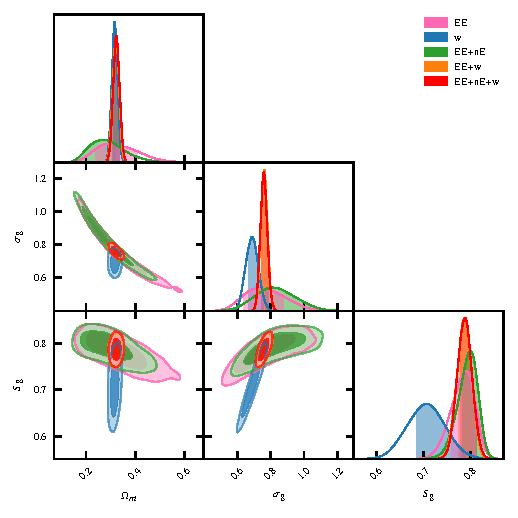
\includegraphics[width=\columnwidth]{Parameter_Plots/omegam_sigma8_s8_blind_A}
		\caption{Constraints on flat $\Lambda$CDM blind A}
		\label{fig:cosmology-params}
	\end{center}
\end{figure}

Fig.~\ref{fig:S8comp} also demonstrates the internal consistency between the different cosmological probes, in terms of their $S_8$ constraints, finding good agreement between the different probe combinations and single probe constraints.  As forecast by \citet{joachimi/etal:inprep}, the addition of the galaxy-galaxy lensing observable adds very little constraining power, with similar results found for the full $3\times2{\rm pt}$ analysis and the combined cosmic shear and clustering analysis.   This is a result of the significant area of BOSS in comparison to KiDS-1000, and the fact that our lack of an accurate non-linear galaxy bias model prohibits the inclusion of large sections of our galaxy-galaxy lensing data vector, shown in Fig.~\ref{fig:Pgk}.   Inspecting the marginalised posterior distributions for an extended set of cosmological parameters in Fig.~\ref{fig:cosmology-params-all}, we find that the addition of the galaxy-galaxy lensing does however serves to moderately tighten constraints on the amplitude of the intrinsic alignment model $A_{\rm IA}$.   

\begin{figure}
	\begin{center}
		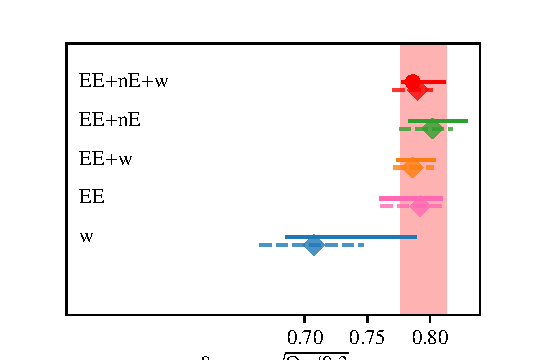
\includegraphics[width=\columnwidth]{Parameter_Plots/S8_comparison_blindA}
		\caption{Constraints on $S_{8}$ blind A}
		\label{fig:S8comp}
	\end{center}
\end{figure}

For the majority of the cosmological parameters shown in Fig.~\ref{fig:cosmology-params-all}, the constraints are uninformed by our choice of prior.  Two key exceptions, however are $n_{\rm s}$ and $h$.  As noted by \citet{troester/etal:2020}, the BOSS galaxy clustering constraints favour a low value for $n_{\rm s}$.   The relatively tight prior adopted in this analysis for $n_{\rm s}$, in Table~\ref{tab:priors}, is therefore very informative, as it is not constrained by KiDS-1000.   BOSS also provides reasonable constraints on $h$, with our $1\sigma$ constraints on $h$ lying within the $h$-prior.   As the marginal probability at the lower prior edge exceeds 20\% of the peak probability, however we consider this parameter unconstrained, setting only an upper limit with $h < X \pm Y$.

\begin{figure*}
	\begin{center}
		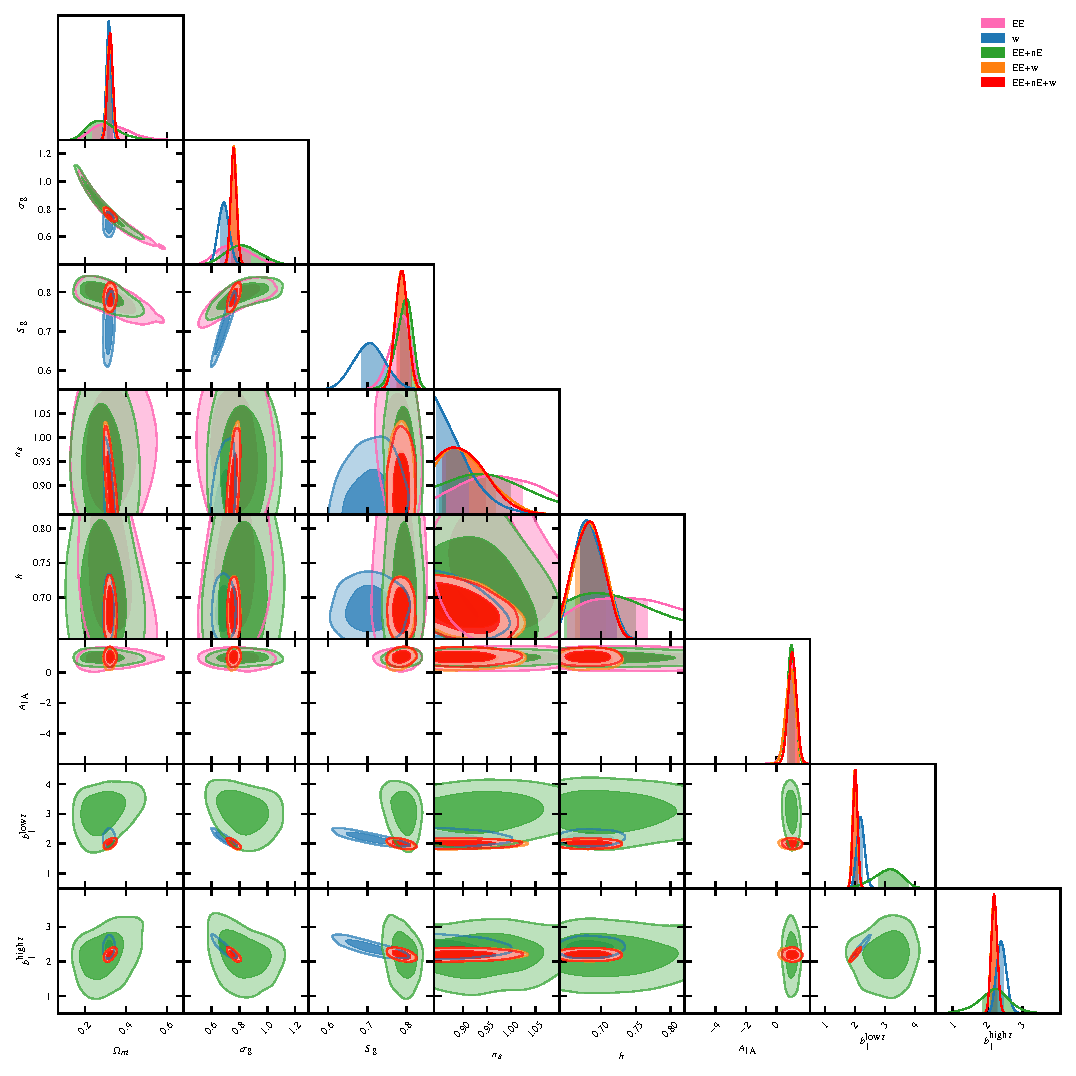
\includegraphics[width=\textwidth]{Parameter_Plots/omegam_sigma8_s8_ns_h_a_ia_b1l_b1h_blind_A}
		\caption{Constraints blind A}
		\label{fig:cosmology-params-all}
	\end{center}
\end{figure*}


\begin{table}
	\begin{center}
		\caption{Goodness of fit for blind A}
		\label{tab:goodness-of-fit}
\begin{tabular}{lrcl}
    \toprule
    Probe             & $\chi^2$       & DoF       & $p$-value   \\
    \midrule
	EE               & $< 156.3$ & $120-4.5$ & 0.007 \\
	w                & $< 176.0$ & $168-13$ & 0.119 \\
	EE+nE            & $< 187.7$ & $142-18$ & 0.000 \\
	EE+w             & $< 327.2$ & $288-20$ & 0.008 \\
	EE+nE+w          & $371.3$ & $310-20$ & 0.001 \\

    \bottomrule
\end{tabular}
	\end{center}
\end{table}


\subsection{Comparison with Planck}
\label{sec:planck_comp}
